\chapter{System Design and Architecture}

\section{System Overview}

The Institutional Recruitment Portal is built using a modern three-tier architecture, designed for scalability, security, and maintainability. The system consists of a presentation layer (React SPA), a business logic layer (Node.js/Express API), and a data layer (MongoDB). The entire system is containerized using Docker, with Nginx serving as a reverse proxy and static file server.

Figure~\ref{fig:architecture} illustrates the high-level architecture. The frontend communicates with the backend via RESTful APIs using JSON for data exchange. The backend handles authentication, authorization, file processing, and database interactions.

\begin{figure}[htbp]
  \centering
  \begin{tikzpicture}[
    box/.style  = {draw, rectangle, rounded corners=3pt, thick,
                   minimum width=6cm, minimum height=1.3cm,
                   align=center, font=\small},
    arr/.style  = {-{Stealth[scale=1.1]}, thick},
    note/.style = {font=\footnotesize\itshape, fill=white, inner sep=2pt}
  ]
    \node[box, fill=gray!20]   (browser) at (0, 7.8) {Browser};
    \node[box, fill=cyan!20]   (nginx)   at (0, 5.6)
          {Nginx\\[1pt]{\footnotesize serves React SPA \& Static Assets}};
    \node[box, fill=green!20]  (express) at (0, 3.6)
          {Node.js\,/\,Express\\[1pt]{\footnotesize REST API Server}};
    \node[box, fill=orange!20] (mongo)   at (0, 1.6)
          {MongoDB\\[1pt]{\footnotesize Document Store}};

    \draw[arr] (browser) -- node[note,right]{HTTP\,/\,JSON}         (nginx);
    \draw[arr] (nginx)   -- node[note,right]{\texttt{/api/*} proxy}  (express);
    \draw[arr] (express) -- node[note,right]{Mongoose ODM}           (mongo);

    \begin{scope}[on background layer]
      \node[draw=blue!50, dashed, line width=1.1pt, rounded corners=8pt,
            fill=blue!4, inner xsep=18pt, inner ysep=18pt,
            fit=(nginx)(express)(mongo),
            label={[blue!60, font=\small\bfseries]above:Docker Compose}] {};
    \end{scope}
  \end{tikzpicture}
  \caption{Three-tier architecture of the Recruitment Portal.}
  \label{fig:architecture}
\end{figure}

\section{User Roles and Access Control}

The system implements Role-Based Access Control (RBAC)~\cite{Sandhu1996} with three distinct portals:

\begin{enumerate}
  \item \textbf{Student (Applicant) Portal:} Allows candidates to register, browse project listings, and submit applications. Applicants can track the status of their submissions and manage their profiles.
  
  \item \textbf{Professor Portal:} Provides tools for professors to create and manage project advertisements. Professors can view detailed applicant profiles, download uploaded documents, and update the recruitment status for each applicant.
  
  \item \textbf{Admin Portal:} Offers high-level oversight, including professor management (approving/blocking accounts), project moderation, and global application tracking.
\end{enumerate}

Table~\ref{tab:roles} summarizes the permissions and primary capabilities for each role.

\begin{table}[H]
  \centering
  \caption{User roles and primary capabilities in the Recruitment Portal.}
  \label{tab:roles}
  \begin{tabularx}{\textwidth}{lX}
    \hline
    \textbf{Role} & \textbf{Primary Capabilities} \\
    \hline
    Administrator & Full system access; Professor account approval; Project moderation; Global application tracking; System configuration. \\
    Professor     & Create and manage projects; View applicant profiles; Download application ZIPs; Export CSV data; Update application status. \\
    Student       & Register and manage profile; Browse active projects; Submit project applications; Upload documents; Track status. \\
    \hline
  \end{tabularx}
\end{table}

\section{Database Design}

MongoDB is used for its flexible schema, which is ideal for handling varying project requirements and applicant data. The primary collections are:

\begin{itemize}
  \item \textbf{Users:} Stores authentication credentials, roles, and basic profile information.
  \item \textbf{Professors:} Extends the User model with department and designation details.
  \item \textbf{Projects:} Contains project codes, titles, descriptions, deadlines, and the ID of the owning professor.
  \item \textbf{Applications:} Links students to projects and professors. It stores the applicant's name, submitted form data, application status, and paths to uploaded documents.
\end{itemize}

Table~\ref{tab:collections} provides a summary of the MongoDB collections and their purposes.

\begin{table}[H]
  \centering
  \caption{Summary of MongoDB collections in the Recruitment Portal.}
  \label{tab:collections}
  \begin{tabularx}{\textwidth}{llX}
    \hline
    \textbf{Collection} & \textbf{Est.\ Docs} & \textbf{Description} \\
    \hline
    Users               & Per system user     & Authentication and role-based access data. \\
    Professors          & Per faculty         & Extended profile for faculty members. \\
    Projects            & Per listing         & Project details, requirements, and deadlines. \\
    Applications        & Per submission      & Student data linked to specific projects. \\
    \hline
  \end{tabularx}
\end{table}

\section{File Storage Architecture}

A key architectural decision was the implementation of a structured local filesystem storage system using Multer. Instead of relying on external cloud storage, the system organizes files in a hierarchical directory structure on the server:

\begin{lstlisting}[float=htbp, language=bash, caption={Uploads directory structure.}]
uploads/
|-- <projectCode>/
|   |-- <applicantName>_<serialNumber>/
|   |   |-- <applicantName>_<serial>_photo.jpg
|   |   |-- <applicantName>_<serial>_resume.pdf
|   |   `-- <applicantName>_<serial>_id_proof.pdf
\end{lstlisting}

This structure ensures that files are easily locatable, collision-resistant, and can be efficiently zipped for bulk download.

\section{Security Architecture}

The system follows a security-first approach:

\begin{itemize}
  \item \textbf{Authentication:} Stateless authentication using JWT.
  \item \textbf{Password Hashing:} Secure hashing using bcrypt.
  \item \textbf{Input Validation:} All API endpoints use \texttt{express-validator} for strict schema enforcement.
  \item \textbf{CORS:} Restricts API access to authorized origins.
  \item \textbf{Static Serving:} Nginx serves the frontend and handles the reverse proxying to the backend, hiding the internal API structure.
\end{itemize}

\section{API Design}

The backend exposes a RESTful API following standard HTTP conventions~\cite{Fielding2000}. Table~\ref{tab:api} lists the major route groups.

\begin{table}[H]
  \centering
  \caption{Principal REST API route groups in the Recruitment Portal.}
  \label{tab:api}
  \begin{tabularx}{\textwidth}{llX}
    \hline
    \textbf{Prefix} & \textbf{Method(s)} & \textbf{Description} \\
    \hline
    \texttt{/api/auth}         & POST           & Login, registration, password management. \\
    \texttt{/api/users}        & GET, PUT       & User profile and account management. \\
    \texttt{/api/professors}   & GET, POST, PUT & Professor onboarding and moderation. \\
    \texttt{/api/projects}     & GET, POST, DELETE & Project listing lifecycle. \\
    \texttt{/api/applications} & GET, POST, PUT & Application submission and status tracking. \\
    \texttt{/api/admin}        & GET, PUT       & System-wide oversight and dashboard data. \\
    \hline
  \end{tabularx}
\end{table}

\section{User Interface Design}

The Recruitment Portal features a clean, professional interface tailored for each user role. The Student dashboard provides a clear overview of available projects, while the Admin dashboard focuses on system-wide statistics and management.

\begin{figure}[H]
  \centering
  \setlength{\fboxsep}{0pt}
  \setlength{\fboxrule}{0.2pt}
  \fbox{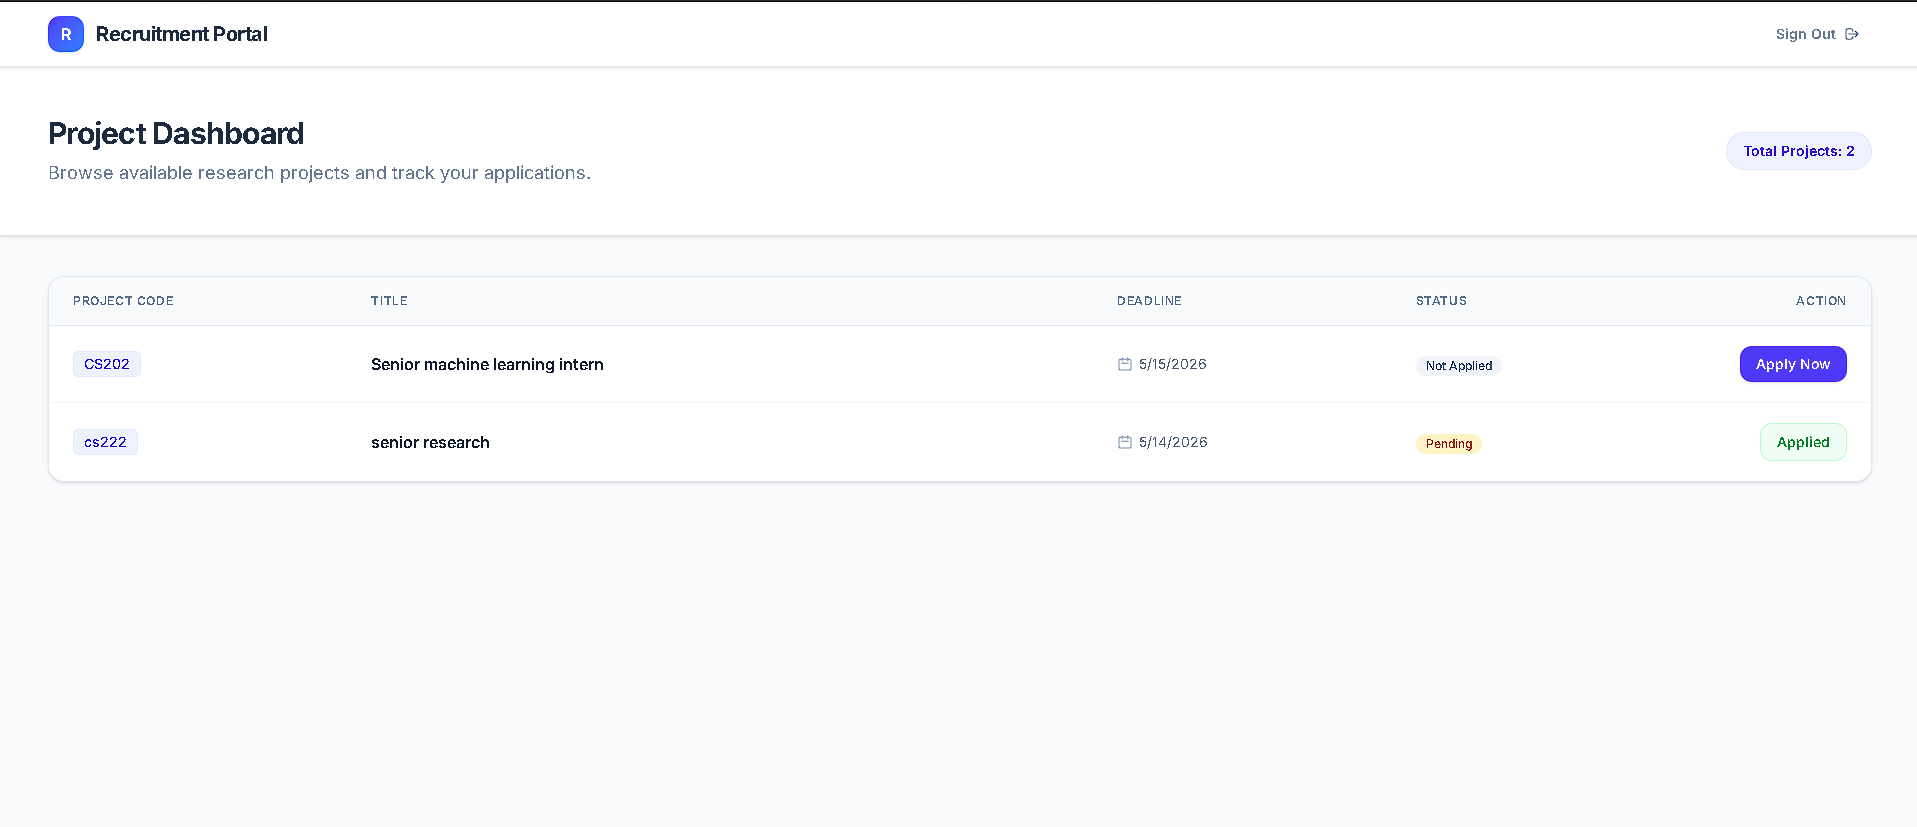
\includegraphics[width=0.85\textwidth]{figures/student_dashboard.png}}
  \caption{Student dashboard showing active project listings and application status.}
  \label{fig:student_dash}
\end{figure}

\begin{figure}[H]
  \centering
  \setlength{\fboxsep}{0pt}
  \setlength{\fboxrule}{0.2pt}
  \fbox{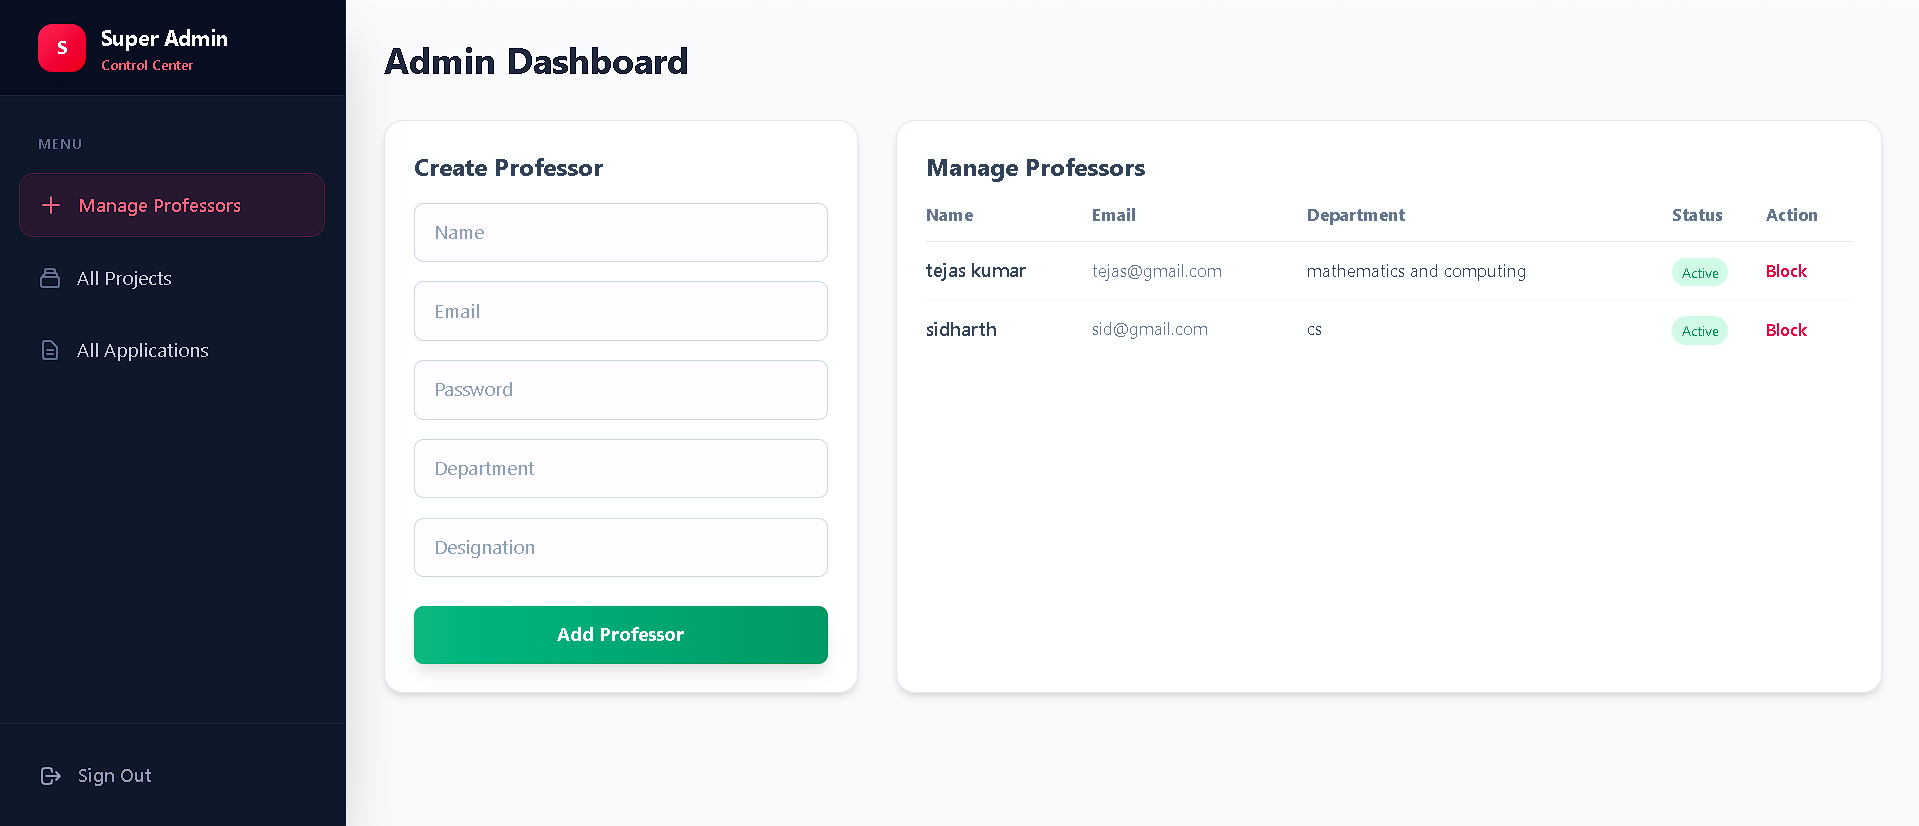
\includegraphics[width=0.85\textwidth]{figures/admin_dashboard.png}}
  \caption{Admin dashboard providing an overview of total professors, projects, and applications.}
  \label{fig:admin_dash}
\end{figure}

\begin{figure}[H]
  \centering
  \setlength{\fboxsep}{0pt}
  \setlength{\fboxrule}{0.2pt}
  \fbox{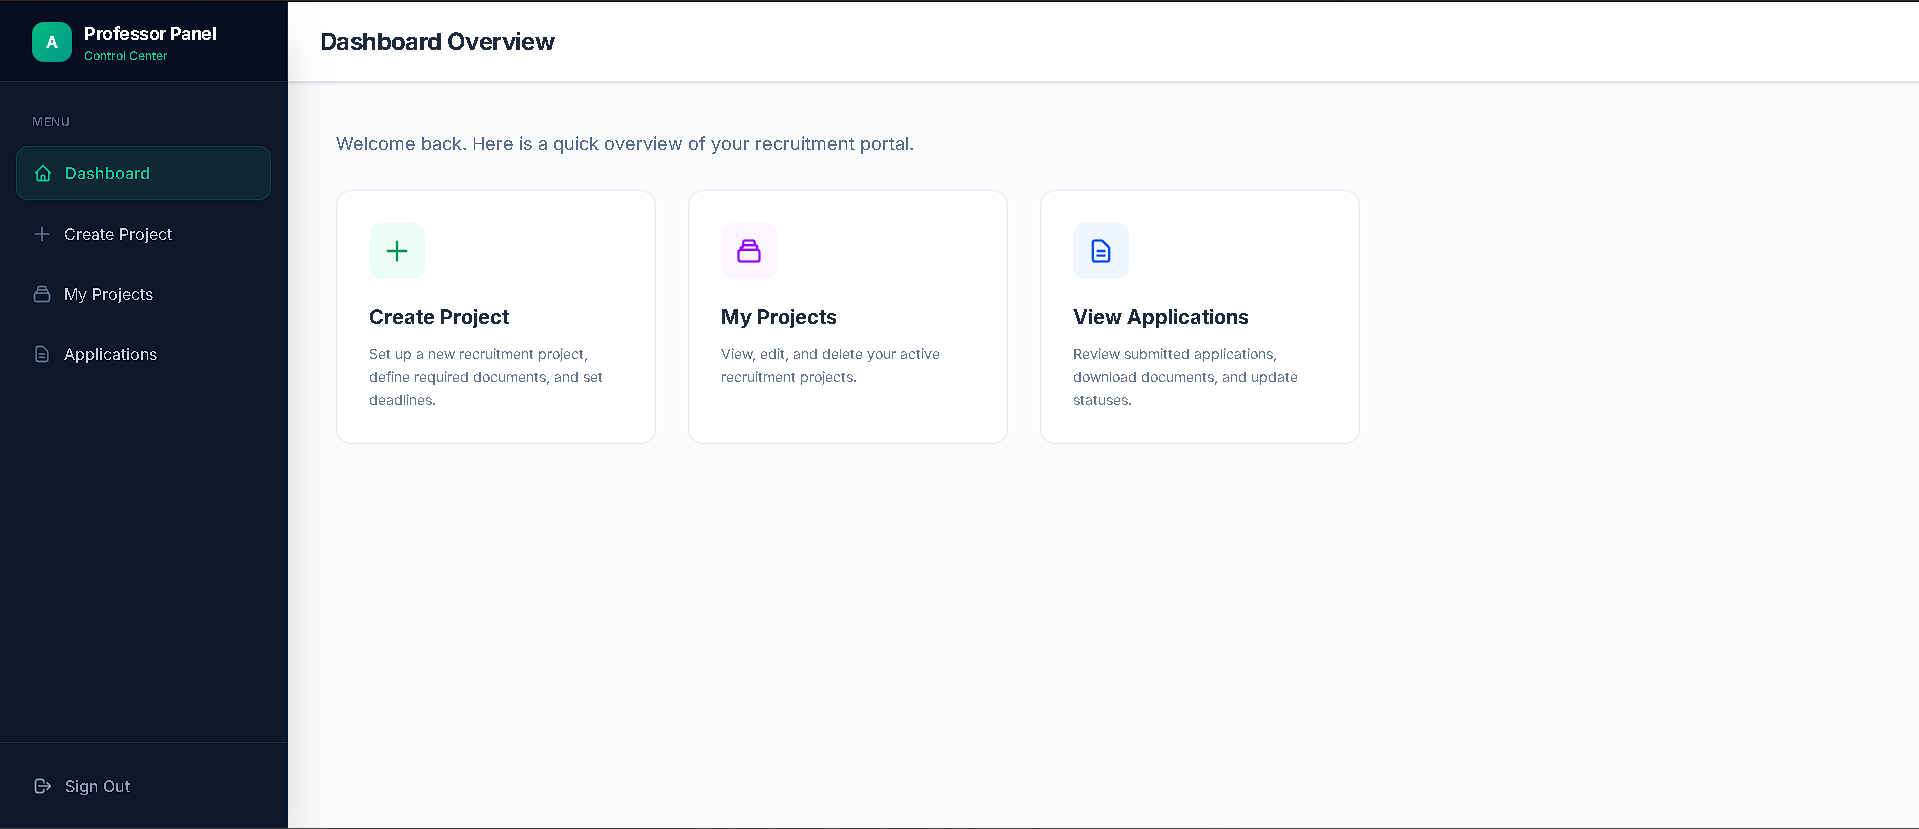
\includegraphics[width=0.85\textwidth]{figures/professor_dashboard.png}}
  \caption{Professor dashboard providing a summary of managed projects and application statistics.}
  \label{fig:prof_dash}
\end{figure}
